\documentclass{bioinfo}

\usepackage{ulem}
\newcommand{\SR}[2]{{\textcolor{blue}{\sout{#1}{#2}}}}
\newcommand{\AC}[2]{{\textcolor{red}{\sout{#1}{#2}}}}

\copyrightyear{2005}
\pubyear{2005}


\begin{document}
\firstpage{1}

\title[short Title]{EBS: an Exact Bayesian Segmentation Algorithm for
  the analysis of biological data-sets}

\author[Sample \textit{et~al}]{Alice Cleynen\,$^{1,*}$, Guillem
  Rigaill\,$^{2}$ and St\'{e}phane Robin\,$^{1}$\footnote{to whom
    correspondence should be addressed}}

\address{$^{1}$AgroParisTech, 16 rue Claude Bernard, 75231 Paris Cedex
  05, France \\ 
$^{2}$URGV, INRA-CNRS-Univ. Evry, 2 Rue Gaston
  Cr\'{e}mieux, 91057 Evry Cedex, France}

\history{Received on XXXXX; revised on XXXXX; accepted on XXXXX}

\editor{Associate Editor: XXXXXXX}

\maketitle


\begin{abstract}

\section{Summary:}
 EBS is an R package for the segmentation of biological data-sets
 (arrayCGH, RNA-seq, etc). It provides, through a Bayesian framework,
 exact quantities such as the posterior distribution of a change-point
 position or an efficient ICL criterion for the selection of the total
 number of change-points. All quantities are computed in quadratic
 time.


\section{Availability:}
EBS is available as an R package from CRAN repositories
(http://cran.r-project.org/web/packages/EBS)


\section{Contact:} alice.cleynen@agroparistech.fr
\end{abstract}

\begin{methods}
\section{Introduction}

Many biological dataset analyses (CNV or transcript
  detection, ...) aim at finding some abrupt change in an ordered signal that
  is typically observed along the genome, and 
can therefore be rephrased as change-point detection
  problems. Most of them do not address
crucial questions such as the quality of the segmentation, or the
uncertainty on the localisation of breakpoints that are useful when
choosing the number of segments, or comparing the segmentation of
different profiles.

Among the few that do are the implementation of Bardy and Hartigan's
Bayesian approach (\texttt{bcp}) that uses MCMC approximation,
\citep{barry_hartigan, bcp_package}, and the frequentist
forward-backward algorithm of \cite{guedon_2008} and constrained-HMM
framework of \cite{Luong_HMM_2012}. Those two later approaches compute
those useful quantities for fixed values of the segment
parameters, and therefore do not account for the uncertainty due
  to their estimation.

EBS is an implementation of the framework described in
\cite{rigaill_exact_2011} which derives \textit{exact} posterior
probabilities of quantities such as the number of segments, the
entropy of a segmentation, or the localisation of the change-points.
The general model can be stated as
  follows: consider data ordered along genomic positions (or probe
  location) $Y = (Y_1, Y_2, \dots Y_n)$. The whole chromosome is
  shattered into successive segments $r$. The observations come from
  some parametric distribution $F$ of which the parameter depends on the
  segment: $i \in r \: \Rightarrow \: Y_i
  \sim F(\theta^r)$.


\section{Available Functionality}
Our approach is valid for all models satisfying the following factoriability
assumption: if $Y$ denotes the data, $m$ a segmentation and $r$ a
segment of $m$,
\begin{equation}
 (H)\quad P(Y,m) = C \prod_{r\in m} a_r P(Y^r|r) \label{factoriability}
\end{equation}
where $P(Y^r|r) =\int P(Y^r|\theta_r)P(\theta_r)d\theta_r $.

This condition is satisfied by the Poisson,
Normal (Heteroscedastic and Homoscedastic with known variance) and
Negative Binomial (with known overdispersion parameter) models which are all included in the
  package. Normal distribution are dedicated to arrayCGH, whereas
Poisson and Negative Binomial are proposed for NGS.

The computation of the quantities of interest rely on the knowledge of $P(Y,K)$
($K$ being the number of segments) that can be computed in quadratic
time as
\begin{equation}
 P(Y,K) = \left[{n-1} \choose{K-1} \right]^{-1} \left(A^K \right)_{1,n+1} \label{Proba}
\end{equation} 
where $A_{i,j}=P(Y^{[\![i,j[\![})$. (See Proposition 2.2
                of \cite{rigaill_exact_2011} for proof). \newline


Table \ref{Tab:01} gives the list of the functions available in the EBS Package. This section describes and illustrates their use with a continued example. 

\subsection{Matrix Construction}

All quantities of interest can be computed using simple operations on the elements of the matrix $A$ of segment probabilities. The function \texttt{EBSegmentation} initializes this matrix with the data according to the user's choice of maximum number of segments and data-model. Each of them is associated with a prior distribution on the parameters (for instance, Gamma for the Poisson model), and the result depends on the value of the hyperparameters. By default \texttt{EBSegmentation} proposes to compute and use data-driven values (see EBS Manual for more details), but the user has the possibility of giving his or her own hyperparameters.

The function returns an object of class \textit{EBS} which contains
the prior information\SR{,}{} matrix $A$, and the two matrices $Li$
and $Col$ in which $k^{th}$ row (respectively column) is the first row
(resp. last column) of the $k^{th}$ power of $A$ ($1\leq k \leq
K_{max}$).  In other words we have: $Li_{i,j}=P([\![Y_0,Y_j[\![,i)$
        and $Col_{i,j}=P([\![Y_i,Y_{n+1}[\![,j)$.

\begin{verbatim}
> set.seed(1)
> require(EBS)
> x<-c(rnbinom(100,0.4,size=0.95),rnbinom(50,0.1,size=0.95),
rnbinom(75,0.4,size=0.95),rnbinom(125,0.1,size=0.95),
rnbinom(75,0.4,size=0.95))
> out <- EBSegmentation(x, model=3, Kmax=20)
\end{verbatim}


\begin{table}[!t]
\processtable{Functions provided by EBS package \label{Tab:01}}
{\begin{tabular}{ll}\toprule
Function Name & Output \\\midrule
 EBSegmentation & Initializes matrix $A$ and its $K_{max}$ first powers\\
 EBSBIC & Computes BIC and chooses the optimal value of K \\
 EBSICL & Computes ICL and chooses the optimal value of K \\
 EBSPostK & Returns the posterior probability of the number of segments\\
 EBSDistrib & Computes the distribution of a change-point\\
 EBSPlotProba & Plots distribution of all change-points for a given K\\\botrule
\end{tabular}}{}
\end{table}




\subsection{Model Selection}

The EBS Package provides two model selection criteria:
\begin{itemize}
\item an exact BIC criterion;
\item and an exact ICL criterion
\end{itemize}
These criteria can be called with functions \texttt{EBSBIC} and
\texttt{EBSICL}.

Considering the segmentation as an unobserved variable, we can use the ICL criterion introduced by \cite{biernacki_assessingmixture_2000} in the context of incomplete data models to select the number of segments. 
The ICL can be written as $ICL(K) = -\log P(Y,K) + \mathcal{H}(K) \label{ICL}$ where
the entropy $\mathcal{H}(K)$ is defined as
\begin{equation}
  \mathcal{H}(K)=-\log \sum_{m\in \mathcal{M}_K} p(m|Y,K) \log p(m|Y,K)
\end{equation}
The entropy can be viewed as a penalty term, which favors
  segmentation with precisely defined change-points location and it
is computed in quadratic time.  Even though in this context the
Bayesian Information Criterion is exact, it tends to
overestimate the number of segments while the ICL performs
better \citep{rigaill_exact_2011}. However, the computation of the BIC
(through function \texttt{EBSPostK}) can be useful for later carrying
analysis such as Bayesian Model Averaging (BMA).
\begin{verbatim}
> print(bic <- EBSBIC(out)$NbBIC)
[1] 6
> print(icl <- EBSICL(out)$NbICL)
[1] 5

\end{verbatim}


\begin{figure}[!h]%figure1
\centerline{\includegraphics[width=5cm,angle=270]{icl-bic.ps}}
\caption{BIC and ICL criteria as a function of the number of segments} \label{fig:01}
\end{figure}






\subsection{Change-point location distribution}

One might be interested in the
distribution of the location of each change-points. Two functions are
implemented to address this question. \texttt{EBSDistrib} returns the
distribution of the $k^{th}$ change-point of a segmentation in $K$
segments. \texttt{EBSPlotProba} plots the distribution of all
$K\!-\!1$ change-points of a segmentation in $K$ segments. The user
has the option to plot those distributions on top of the data.
\begin{verbatim}
> EBSPlotProba(out, icl, data=TRUE)
\end{verbatim}

\begin{figure}[!h]%figure1
\centerline{\includegraphics[width=6cm,angle=270]{my-segmentation.ps}}
\caption{Output of function \texttt{EBSPlotProba}: distribution of the localisation of the change-points on simulated data (right y-axis, blue)}\label{fig:02}
\end{figure}




\section{Conclusion}

An exact computation of many powerful quantities is obtained thanks to
the exploration of the entire segmentation space in a Bayesian
framework adapted to the analysis of NGS and CGH-array data.  It
provides a useful criterion for the selection of the number of
segments, and allows further analysis of variables such as the entropy
or the location of change-points.  Future improvements to the package
may include the calculation of other quantities of
interest, such as the posterior mean of the signal, which would
  provide an estimate of the copy number at a given locus, or of the
  expression level of a given exon.



\section*{Acknowledgement}
We wish to thank Gregory Nuel and Michel Koskas for their help dealing with numerical issues.


%\bibliographystyle{natbib}
%\bibliographystyle{achemnat}
%\bibliographystyle{plainnat}
%\bibliographystyle{abbrv}
\bibliographystyle{bioinformatics}
%
%\bibliographystyle{plain}
%
%\bibliography{Document}


\begin{thebibliography}{}

\bibitem[Barry and Hartigan, 1993]{barry_hartigan} Barry, D., and Hartigan, J. A. (1993) A Bayesian Analysis for Change Point Problems {\it Journal of the American Statistical Association}, {\bf 88} 309-319

\bibitem[Biernacki {\it et~al}., 2000]{biernacki_assessingmixture_2000} Biernacki, C., Celeux, G. and Govaert, G. (2000) Assessing a mixture model for clustering with the integrated completed likelihood, {\it{IEEE} Transactions on Pattern Analysis and Machine Intelligence}, {\bf 22} 719-725.

\bibitem[Erdman and Emerson, 2007]{bcp_package}   Chandra Erdman and John W. Emerson (2007) {\bf{bcp}}: An {R} Package for Performing a Bayesian Analysis
      of Change Point Problems {\it Journal of Statistical Software}, {\bf 3} 1-13

\bibitem[Gu\'{e}don, 2008]{guedon_2008} Gu\'{e}don, Y. (2008) Exploring the segmentation space for the assessment of multiple change-points models. {\it Technical report, Preprint INRIA} {\bf 6619}

\bibitem[Luong {\it et~al}, 2012]{Luong_HMM_2012} Luong, T.~M., Rozenholc, Y. and Nuel, G. (2012) Fast estimation of posterior probabilities in change-point models through a constrained hidden Markov model {http://adsabs.harvard.edu/abs/2012arXiv1203.4394L}.

\bibitem[Rigaill {\it et~al}., 2010]{rigaill_exact_2011} Rigaill, G., Lebarbier, E., Robin, S. (2011) Exact posterior distributions over the segmentation space and model selection for multiple change-point detection problems, {\it Statistics and Computing}, {\bf 22-4}, 917-929.

\end{thebibliography}
\end{methods}
\end{document}
